\documentclass[12pt, a4paper]{report}

\usepackage[T1]{fontenc}
\usepackage[utf8]{inputenc} 
\usepackage[english]{babel}
\usepackage[top=3cm, bottom=3cm, left=2cm, right=2cm]{geometry}
\usepackage{graphics}
\usepackage{graphicx}
\usepackage{eurosym}
\usepackage{soul}
\usepackage{graphicx} %utilisation d'images
\usepackage{amsmath}
\usepackage{relsize}
\usepackage{titlepic}
\usepackage{times}
\usepackage{url}
\usepackage{listings}
\usepackage[]{algorithm2e}
\usepackage{hyperref}
\usepackage[normalem]{ulem}
\usepackage{hyperref}
\usepackage{tocloft}
\usepackage{float}
\usepackage[dvipsnames]{xcolor}
\usepackage[colorlinks = true,
            linkcolor = blue,
            urlcolor  = blue,
            citecolor = blue,
            anchorcolor = blue]{hyperref}

\newcommand{\MYhref}[3][blue]{\href{#2}{\color{#1}{#3}}}%


\begin{titlepage}
\newcommand*{\defeq}{\stackrel{\mathsmaller{\mathsf{def}}}{=}}
\title{\textcolor{BrickRed}
    {\Huge Learn'English}\\ 
    \large \textit{Desktop app for the English module project}}
\author{Pierre-Arnaud BLANC \\ Guillaume GARCIA}
\date{\today}
\titlepic{
\includegraphics[scale=0.5]{images/telecomnancy.png}

\includegraphics[scale=1]{images/universitelorraine.jpg}}
\end{titlepage}


\lstset{
numberstyle=\small, 
frame = single, 
language=C++, 
framexleftmargin=pt,
basicstyle = \footnotesize}

\makeatletter
\DeclareUrlCommand\ULurl@@{%
  \def\UrlFont{\ttfamily\color{blue}}%
  \def\UrlLeft{\uline\bgroup}%
  \def\UrlRight{\egroup}}
\def\ULurl@#1{\hyper@linkurl{\ULurl@@{#1}}{#1}}
\DeclareRobustCommand*\ULurl{\hyper@normalise\ULurl@}
\makeatother


\renewcommand\cftchapfont{\Large\bfseries}
\renewcommand\cftsecfont{\large}

\renewcommand\cftchapafterpnum{\par\addvspace{10pt}}
\renewcommand\cftsecafterpnum{\par\addvspace{6pt}}


\begin{document}
\maketitle
\hypersetup{linkcolor=blue}


\tableofcontents

\newpage
\chapter*{Introduction}
\addcontentsline{toc}{chapter}{Introduction}

\paragraph{}This report presents our application \textit{Learn'English} as part of the TELECOM Nancy English module. The application aims to help the user into learning specific vocabulary, and most of irregular verbs.

\paragraph{}We noticed that the basics, especially irregular verbs and vocabulary, are lacking to most of people who learn English. And as everybody knows, a strong basis is required to improve your level. Therefore, we had the idea of developing a software tool which could make the checking of those bases more playful and convenient for students. Also, in an ergonomic concern, we wanted our application to be the more portable as possible.

\paragraph{}Consequently, we designed two main features in our app. The first one, named \textit{Train your vocabulary}, is a translation exercise in order to make you memorize your own vocabulary sheet. We will talk about those custom training sheets later in this report. The second feature, named \textit{Check your irregular verbs}, allows you to train yourself on more than 150 irregular verbs. You can also custom this session to make a more personal workout.

\paragraph{}The report will first set forth the \textit{User documentation}, explaining precisely how to use correctly the app. Then, it will pose a \textit{Technical presentation}, written in French, where the exact specification of our app is exposed. Finally, after the conclusion, you will be able to see our bibliography and a link to the executable file (binary) and the source code of the app (\textit{GitHub} link).

\newpage
\chapter*{User documentation}
\addcontentsline{toc}{chapter}{User documentation}

\paragraph{}\textit{Learn'English} was designed for training the user on the basics about English language. Thus, two main separate features were built around two simple exercises. These exercises include a vocabulary test, which consists of assembly-line translations of words, and an irregular verbs test, where you are asked to give past forms of different irregular verbs. Moreover, you can load specific training sheets for both exercises, and also store your high scores and compare them to those of other students. Therefore, our software become a real and powerful tool to help students to check their basic knowledge. To ensure that, it uses light databases in CSV format.

\section*{\hspace{0.6cm}Setting up a working session}
\addcontentsline{toc}{section}{Setting up a working session}

\paragraph{}When you launch the app you reach the home window (see \textbf{Picture 1}). Then the app will ask you a username, type the one you want, and click the \textit{Log in} button. It will associate your username to your future high scores and load ancient ones.

\begin{figure}[H]
    \captionof{\textbf{Picture 1}: Home window}
    \centering
    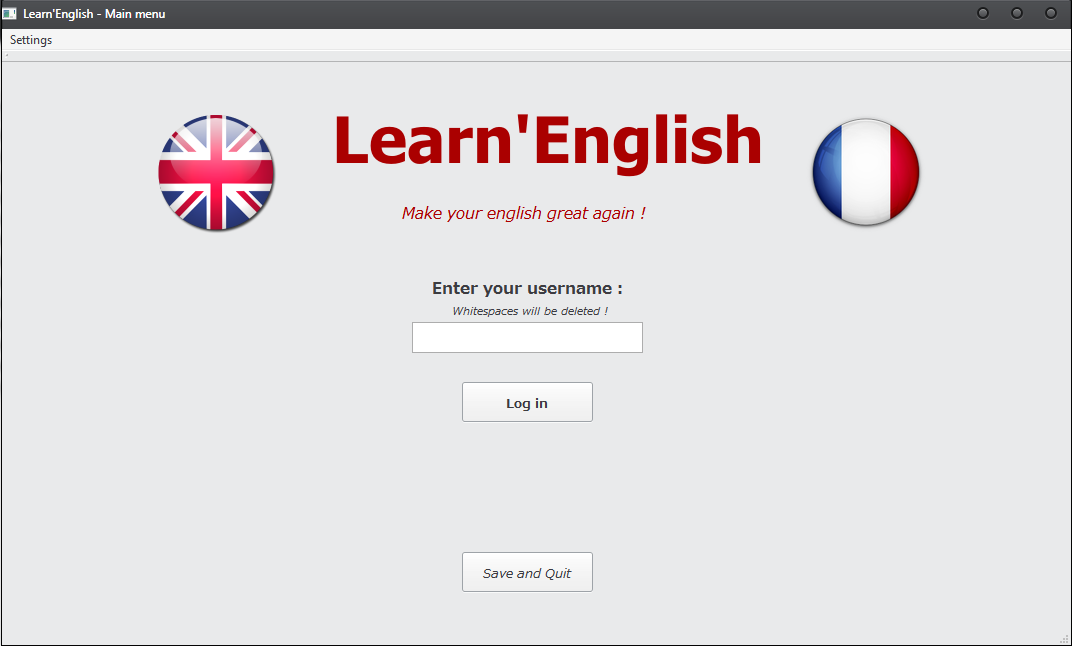
\includegraphics[scale=0.55]{images/home.png}
\end{figure}
\newpage
\paragraph{}Note that if there isn't a file named \textit{saves.csv} (the default save file loaded after logging)  in the same folder as the executable file \textit{learnEnglish.exe} on Windows, or \textit{learEnglish} on Linux, you'll get an error telling you that the could load the save file. If it happens, do not worry and follow these steps:\\
\\
\hspace*{0.5cm}- Click on \textit{Settings} in the menu bar.\\
\hspace*{0.5cm}- Choose \textit{Load save CSV file ...}\\
\hspace*{0.5cm}- Indicate the path (absolute or relative) to a valid save file, in CSV format, then press \textit{OK}.\\
As long as no valid and existing save file is specified, you are not permitted to launch any exercise. This problem of non-existing files could also happen once you launch one of the exercises : the necessary databases are missing. You can solve this problem by a similar way (see \textbf{Picture 2}).

\begin{figure}[H]
    \captionof{\textbf{Picture 2}: Settings in the menu bar}
    \centering
    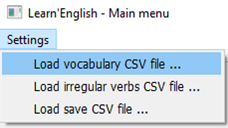
\includegraphics[scale=0.70]{images/menu.png}
\end{figure}

\paragraph{}Since you have downloaded normally the archive containing the app (see the download link in the appendix), you should not get these problems because it provides a save file and a database for each exercise. But your may want to load you own sheets of vocabulary or irregular verbs; that's the point of our tool ! To do that, follow these few steps (see \textbf{Picture 2}):\\
\\
\hspace*{0.5cm}- Click on \textit{Settings} in the menu bar.\\
\hspace*{0.5cm}- Choose \textit{Load vocabulary CSV file ...} or \textit{Load irregular verbs CSV file ...}.\\ A small window will pop up (see \textbf{Picture 3}: example of loading a file for vocabulary training).\\
\hspace*{0.5cm}- Indicate the path to an CSV file corresponding to the desired exercise, then press \textit{OK}.\\

\begin{figure}[H]
    \captiono{\textbf{Picture 3}: Loading a custom sheet for the vocabulary training.}
    \centering
    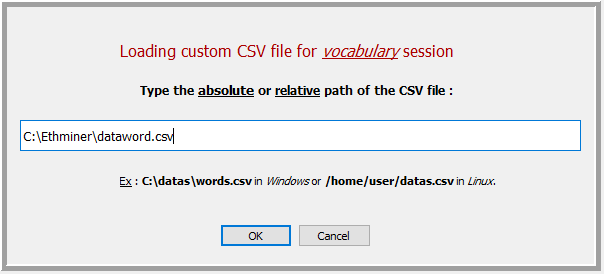
\includegraphics[scale=0.55]{images/load.png}
\end{figure}

\paragraph{}Once you are logged in and all the settings are correctly set up, two start-buttons appear: you are ready to launch an exercise. If your username already exists in the save file, the app will load your own high scores for both exercises and display them above the two buttons (see \textbf{Picture 4}). To start a training session, just click on the corresponding button. Note that if you increase your highscore in an exercise, and you want to update it on the home window, just push the button refresh (the one with the icon).
\begin{figure}[H]
    \captionof{\textbf{Picture 4}: Logged in and ready to go!}
    \centering
    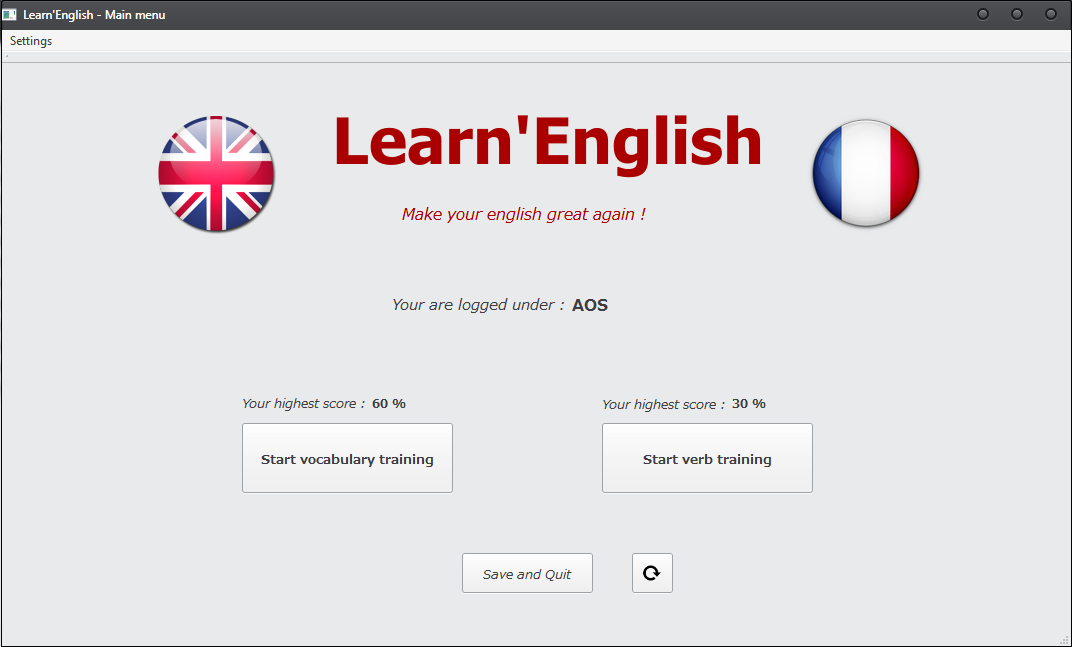
\includegraphics[scale=0.55]{images/homelogged.png}
\end{figure}


\paragraph{}To close the app, just press the \textit{Save and Quit} button. It will automatically store your highscores in the CSV save file (see \textbf{Picture 4}). To know more about CSV files, refer to the \textbf{Technical documentation}.

\paragraph{}Be aware that if you have not configured correctly the app you will not be able to launch any exercise since they use external files (CSV format) to generate words and irregular verbs.


\newpage
\section*{\hspace{0.6cm}Vocabulary training}
\addcontentsline{toc}{section}{Vocabulary training}

\paragraph{}At this step, you should have already configured correctly the databases. If not, an error message might appear once you click on the \textit{I'm ready !} button, then you should read the solution in the previous section.
\paragraph{}Once the exercise is launched, the app will ask you to translate a given English word into its main meaning in French. Type it in the line-edit, then push the \textit{Validate} button or press Enter key. If it's correct you'll see a \textit{\textcolor{ForestGreen}{Right !}} just below the line-edit. If not, a \textit{\textcolor{BrickRed}{Wrong ...}} will appear and the app will print the solution (see \textbf{Picture 5}).

\paragraph{}For each correct answer, you earn one point. You don't earn any point for a wrong one. You score is displayed and updated all the time in the right corner of the window. A progress bar indicates you how many words are left. When you have validated -or not a word, just click the \textit{Next !} button, another word will be picked up randomly. Words that have already been checked are not showed anymore until the end of the session: a given word appears just once during a session.

\begin{figure}[H]
    \captionof{\textbf{Picture 5}: Vocabulary exercise sample}
    \centering
    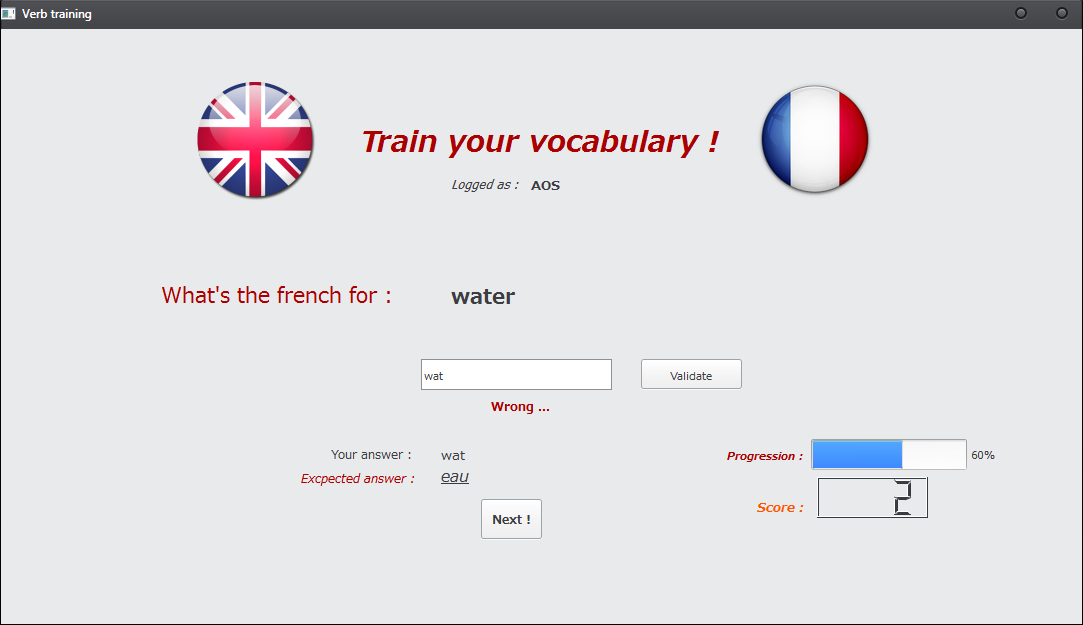
\includegraphics[scale=0.55]{images/vocab.png}
\end{figure}

\paragraph{}The provided database for vocabulary \textit{datawords.csv} contains almost \textbf{40} couples of words. This is a light sheet, but the user can enlarge this database up to 2000 couples of words (limit fixed by the compiler in our code). Once you finish the exercise, a new screen pops up. Refer to the \textbf{End of session} section for more info about that.
\newpage
\section*{\hspace{0.6cm}Check your irregular verbs}
\addcontentsline{toc}{section}{Check your irregular verbs}

\paragraph{}As in the \textbf{Vocabulary training} section, just push the \textit{I'm ready !} button. If an error message is printed, refer to the solution in the \textbf{Setting up a working session} section.

\paragraph{}The process here is similar to the vocabulary exercise. The app shows an irregular verb in its infinitive form. Type its preterit form in the first line-edit and the past participle form in the second one, then push \textit{Validate} button or press Enter key. If a form is correct you'll see a \textit{\textcolor{Green}{Right !}} just below the corresponding line-edit. If not, a \textit{\textcolor{Red}{Wrong ...}} will appear and the app will print the solution below the wrong answer. The French translation of the verb is also displayed, just for information, on the right frame (see \textbf{Picture 6}).

\paragraph{}For each correct answer, you earn one point. You don't earn any point for a wrong one; thus you may earn up to 2 points per irregular verb. You score is displayed and updated all the time in the right corner of the window. A progress bar indicates you how many verbs are left. When you have validated -or not a pair of forms, just click the \textit{Next !} button, another irregular verb will be picked up randomly. Verbs that have already been checked are not showed anymore until the end of the session: a given verb appears just once during a session.

\begin{figure}[H]
    \captionof{\textbf{Picture 6}: Irregular verbs exercise sample}
    \centering
    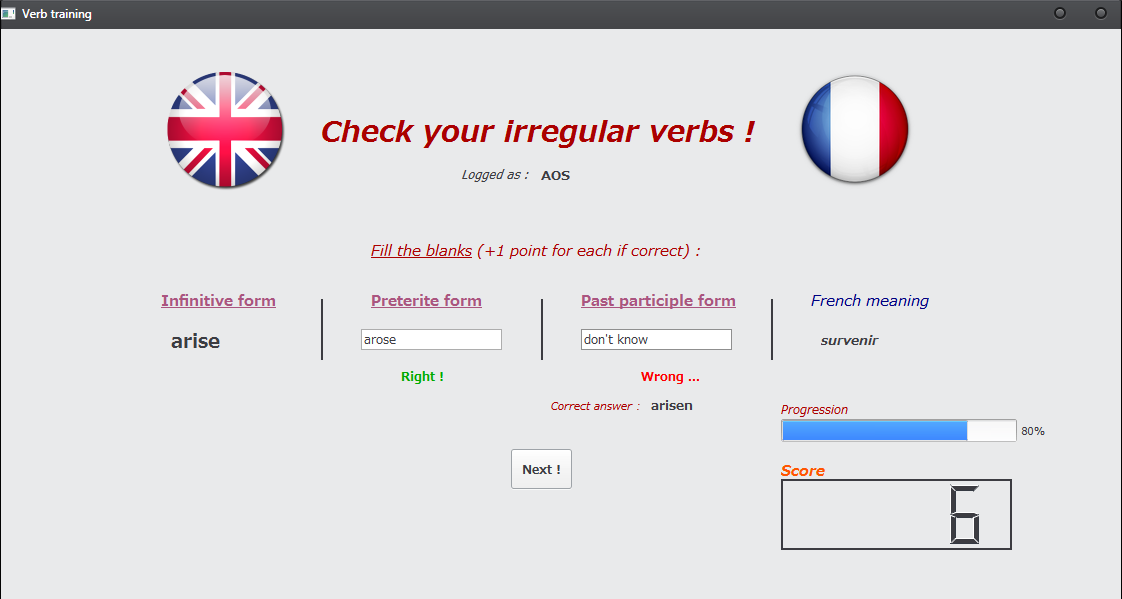
\includegraphics[scale=0.55]{images/verbs1.png}
\end{figure}

\paragraph{}The provided database for irregular verbs \textit{dataverb.csv} contains exactly \textbf{152} irregular verbs. Thought this is a large sheet, the user can enlarge this database up to 2000 irregular verbs with its three forms plus the French translation (limit fixed by the compiler in our code). Despite this limit, there are about 200 irregular verbs in English in normal use... Once you finish the exercise, a new screen pops up. Refer to the \textbf{End of session} section for more info about that.

\newpage
\section*{\hspace{0.6cm}End of a session}
\addcontentsline{toc}{section}{End of a session}

\paragraph{}When you finish an exercise, a special ending screen is displayed (see \textbf{Picture 7}). It's almost the same for both training. It shows your final score, and your percentage calculated by the ratio of your final score to the maximum score reachable (which is also printed). The highest score recorded in the save file for this exercise is also displayed, and below it you will see the username of the best player associated to this highscore.

\paragraph{}Once you're done, just click ont the \textit{Got it !} button. This will close this training and you'll reach the home windows. To update your new highscore on the screen, juste press the \textit{Refresh} button (the one with the arrow) in the home window. Once an exercise is done, you cannot re-launch it until you quit the app, by clicking the \textit{Save and Quit} button (see \textbf{Picture 4}). It saves your highscores only if they are better than the ancien ones.

\begin{figure}[H]
    \captionof{\textbf{Picture 7}: End of session, print scores}
    \centering
    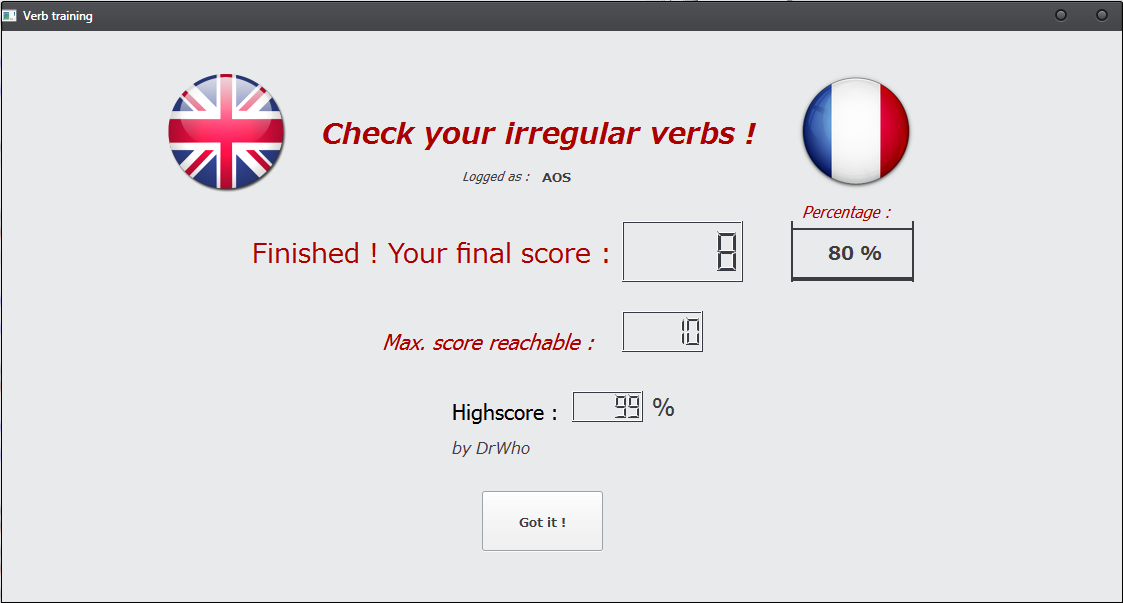
\includegraphics[scale=0.55]{images/high.png}
\end{figure}

\newpage
\chapter*{Technical documentation}
\addcontentsline{toc}{chapter}{Technical documentation}

\section*{\hspace{0.6cm}Conception}
\addcontentsline{toc}{section}{Conception}

\paragraph{}Le choix de conception étant totalement libre, nous avons d'entrée de jeux choisi de sortir des sentiers battus. Un des langages les plus utilisés aujourd'hui dans les entreprises de software est le C++, c'est aussi un langage très répandu dans le \textit{Logiciel Embarqué}, ce qui correspond à notre approfondissment (LE). Nous n'avons donc pas hésité à choisir le C++, afin de nous former dans ce langage. Une telle formation est un atout non négligeable sur un C.V. de jeune ingénieur spécialisé en logiciels embarqués.

\paragraph{}Bien évidemment, concevoir une application bureau, donc graphique, est une tâche bien plus ardue que le développement d'un simple programme en ligne de commande. Les bibliothèques standardes \textit{GNU/Linux} étant relativement pauvres et peut satisfaisantes pour notre objectif, nous avons décidé d'utiliser un \textbf{framework}, c'est-à-dire un cadre applicatif ou une infrastructure de développement, bien connu dans le domaine industriel et relativement bien répandu. Ce framework s'appelle \textbf{\textit{Qt}}. Nous l'avons utilisé dans sa version 5.8 (dernière version stable en date). Ce framwork est spécialisé dans le développement d'application bureau. De plus, \textbf{\textit{Qt}} est disponible aussi bien sur \textit{Linux} que sur \textit{Windows} (nous avons développé notre application sur les 2 systèmes d'exploitations). Il était ainsi beaucoup confortable de concevoir notre application.

\paragraph{}L'autre avantage de \textbf{\textit{Qt}} est la portabilité des applications construites avec. En effet, il est possible, lors du déploiment de l'application, de compiler une release pour \textit{Windows}, et une pour \textit{Linux}. Pour \textit{Windows}, seule une poignée (17) de fichiers \textit{DLL} (des bibliothèques windows) sont requis pour faire fonctionner l'application, et ils sont fournis dasn l'archive du lien de téléchargement. En revanche pour \textit{Linux}, il est nécessaire d'avoir installé a minima le paquet \textit{qt5-default} (pour \textit{Ubuntu/Debian}).

\paragraph{}En addition de ce framework, nous avons utilisé l'IDE (\textit{Integrated Developpement Environment} dédié à \textbf{\textit{Qt}} : \textbf{\textit{Qt Creator}}. Cet IDE s'utilise un peu comme Microsoft Visual Studio C++, c'est-à-dire que son gros atout réside en la possibilité de concevoir les parties graphiques (appelés \textit{Widgets}, cela comprend les boutons, les labels, les line-edit, les barres de progression, etc...) directement depuis l'IDE en plaçant à la souris les éléments sur les différentes fenêtres de l'application. Cela est rendu possible par son outil intégré appelé \textit{Qt Designer} (c.f. \textbf{Image 8}).

\begin{figure}[H]
    \captionof{\textbf{Image 8}: Qt Designer, l'outil de Qt Creator pour créer simplement des interfaces graphiques}
    \centering
    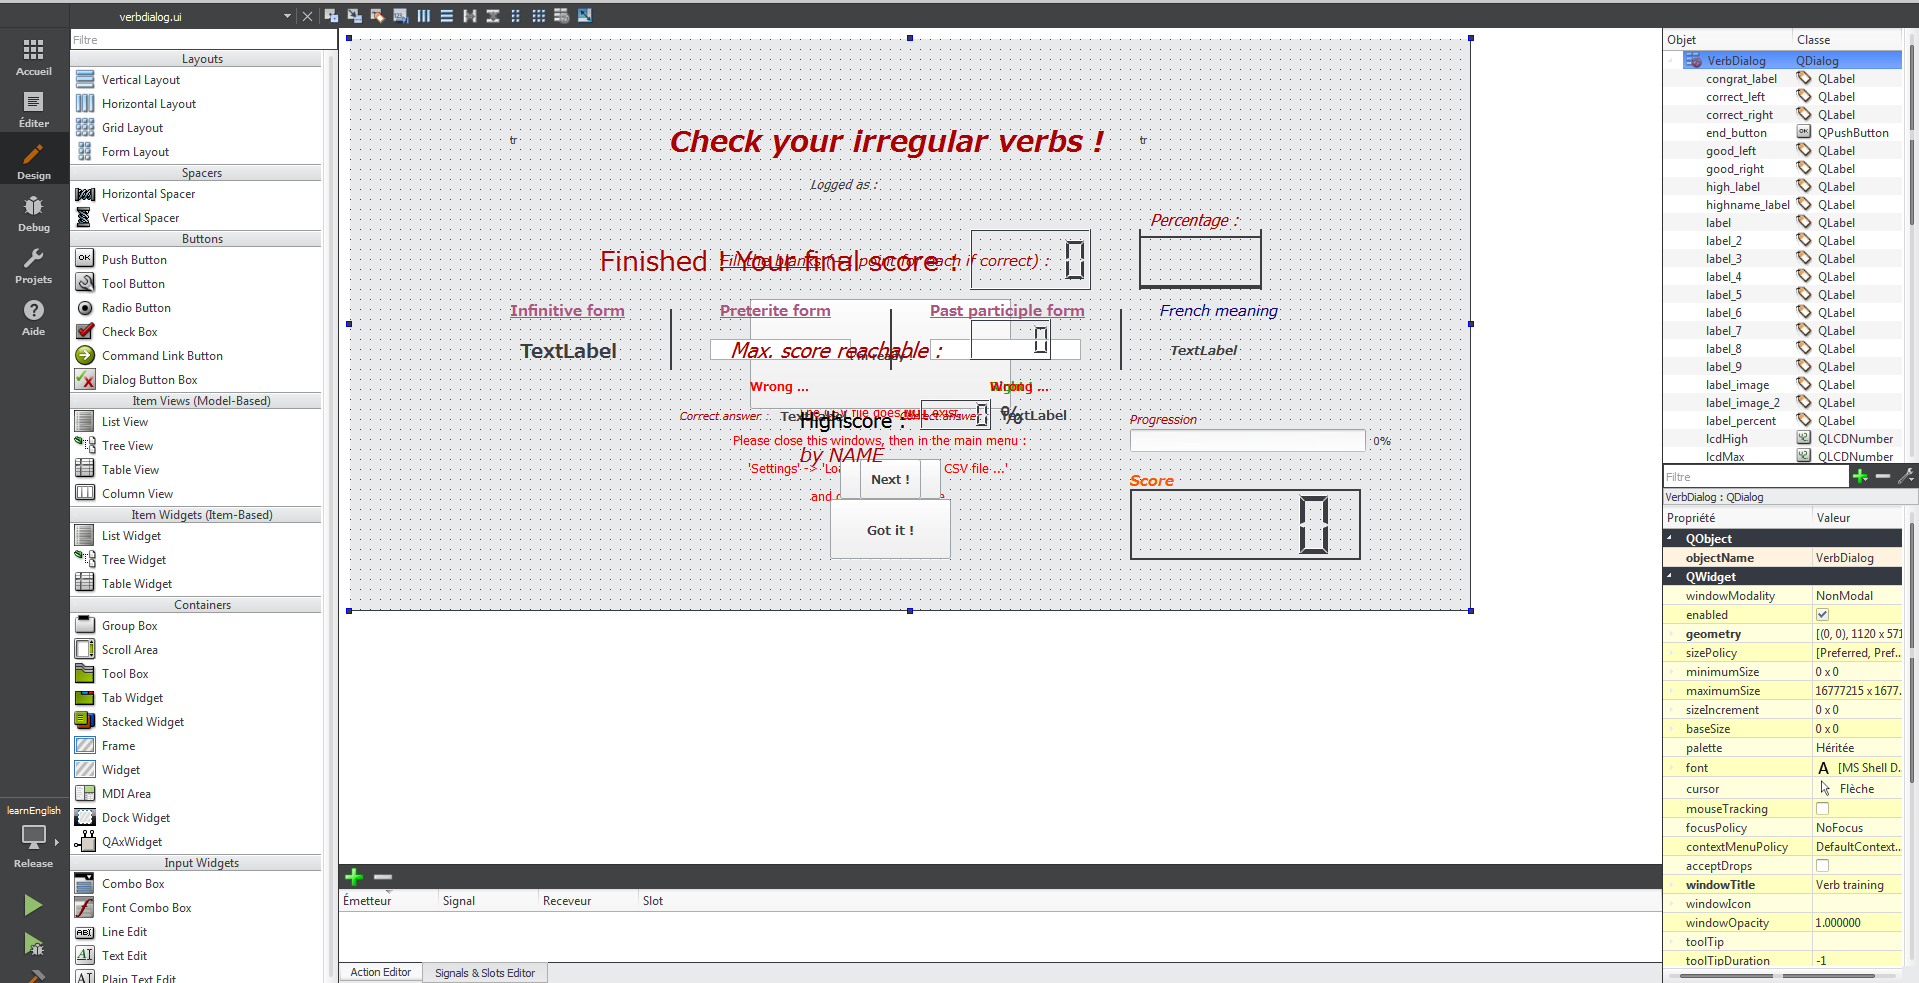
\includegraphics[scale=0.34]{images/qtcreator.png}
\end{figure}

\paragraph{}Bien que la programmation brute ait été largement allégée par ce procédé, il a quand même fallu implémenter le moteur de l'application. Comme vous pouvez le voir sur l'\textbf{Image 8}, tous les \textit{Widgets} se superposent indifférement sur la fenêtre. Il faut dire à l'application quand ils doivent apparaitre, disparaitre, afficher telle ou telle valeur ou chaine de caractères.

\paragraph{}Pour réaliser le moteur de production de verbes irréguliers et mots de vocabulaire, nous avons dû concevoir un générateur aléatoire à exclusion; c'est-à-dire un générateur aléatoire qui exclut de sa génération les mots ou verbes déjà tirés. Pour cela nous avons créé une petite fonction \textit{randAB(int min, int max)} qui génère aléatoirement un entier entre deux bornes passées en paramètres. Cette fonction est ensuite utilisée pour générer aléatoirement un indice du tableau de mots/verbes chargé en mémoire. Suite à quoi cet indice est utilisé pour piocher dans ce tableau de mots/verbs, puis il est ajouté à un tableau d'exclusion (de type tableau d'entier). Chaque fois qu'un nouvel indice est généré, on vérifie qu'il n'existe pas déjà dans ce tableau d'exclusion. Si il a déjà été tiré, un nouvel indice est généré, sinon il est utilisé pour piocher dans le tableau de mots/verbes, et ainsi de suite. Lorque la taille du tableau d'exclusion atteint le nombre de ligne du tableau de mots/verbes, on en déduit que c'est la fin de l'exercice.

\paragraph{}Afin de réaliser un travail d'équipe efficace, nous avons utilisé le gestionnaire de version \textbf{git}, extrêmement répandu et maîtrisé par nous-même. Nous avons hébergé notre dépôt sur \MYhref{https://github.com/AOSauron}{\textit{GitHub}}. Le projet est d'ailleurs placé sous une Licence Public Générale GNU v3.0.
\newpage
\paragraph{}En ce qui concerne les différentes bases de données, nous avons tenu compte du fait que ces dernière étaient plutôt simples et légères. De plus, nous voulions appuyer sur la partie "personnalisable" des séances de révision. Il nous fallait donc une structure de donnée simple. Elle fut toute trouvée : le format CSV. Très répandue, elle a également l'avantage d'être facile de conception ou de modification. LibreOffice ou Microsoft Excel voire un simple éditeur de texte suffisent pour cela.


\begin{figure}[H]
    \captionof{\textbf{Image 9}: Structure d'un CSV pour les verbes irréguliers}
    \centering
    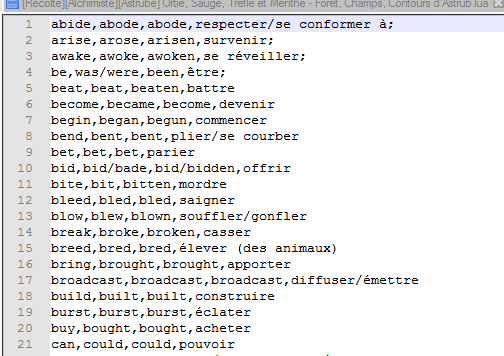
\includegraphics[scale=0.80]{images/csv.png}
\end{figure}

\paragraph{}Pour construire un base de données adaptée aux verbes irréguliers, il suffit de mettre sur chaque ligne les trois formes et la traduction, sans espaces, et séparés par des virgules (c.f. \textbf{Image 9}). La forme de chaque ligne est donc la suivante :
\[infinitif,preterit,participePasse,traduction\]



\paragraph{}La base de données des mot de vocabulaire est plus simple. Simplement le mot anglais et la traduction française séparés par une virgule sur chaque ligne. La forme d'une ligne est donc la suivante :
\[motAnglais,traductionFr\]

\newpage
\section*{\hspace{0.6cm}Difficultés rencontrées}
\addcontentsline{toc}{section}{Difficultés rencontrées}

\paragraph{}La première difficulté à laquelle nous avons été rapidement confrontés a été la nouveauté du langage et du framework. Le C++ n'est pas réputé pour être un langage facile d'apréhension. En plus de cela il a fallu ingérer une quantité relativement important de documentation technique sur le framework \textbf{\textit{Qt}} et sur l'IDE \textbf{\textit{Qt Creator}}. Il fut plus facile de gérer l'IDE, qui est conçu pour être ergonomique.

\paragraph{}Le C++ a dû être utilisé dans sa forme Orientée Objet. Bien que nous soyons bien formés pour ce type de paradigme de programmation, notamment grâce au \textit{Java}, les différences de langage, de sémantiques, et de conceptions nous ont posé problème tout le long du développement. Nous avons néamoins réussie à surmonter ces épreuves, notamment grâce à nos connaissances en C.

\paragraph{}Devant la colossale charge de travail nous avons décidé de séparer intelligemment le code en plus ieurs parties. Une première partie gère la fenètre d'accueil. Deux autres parties gèrent indépendamment la fenêtre de vocabulaire et la fenêtre de verbes iréguliers. Enfin, une dernière partie, qui elle n'est pas orienté objet (n'est pas une classe, se comporte comme un fichier C, langage que nous maitrisons), qui fournit plusieurs fonctions utiles aux trois autres parties. Ce ne fut pas une tâche facile pour des novices en la matière tels que nous.

\paragraph{}Une autre difficulté a été de réussir à créer le générateur aléatoire à exclusion. Beaucoup d'erreurs à l'execution (des \textit{overflow}), dues à des mauvaises et hasardeuses indexations, nous ont frenés dans le développement.

\paragraph{}Il a également été difficile de construire une base de données pour le vocabulaire qui ne soit pas [trop] ambiguë. La polysémie des mots augment de façon exponentielle la difficulté du problème. De ce fait cette base de données ne fait actuellement que 40 lignes (soit 40 traduction possibles). Nous avons été obligé de conserver un moteur de vérification simple pour ne pas faire exploser la densité du code, et la complexité en mémoire et en temps à l'execution.

\paragraph{}Pour finir, nous avons dû créer un parseur de fichiers CSV (nos bases de données). Ne connaissant pas bien le C++ avec le framework \textbf{\textit{Qt}}, il fut plutôt difficile d'implémenter correctement ce parseur. Ce parseur s'étend également à toutes les line-edit; cela consiste en l'élimination des virgules et des espaces, pour ne pas corrompre le fichier des sauvegarde lors du \textit{Save and Quit}. Rappelons qu'une virgule marque la séparation des éléments dans un CSV.

\newpage
\chapter*{Conclusion}
\addcontentsline{toc}{chapter}{Conclusion}

\paragraph{}The fact that the topic allowed us a free design for the application was a real boon for us. Therefore we could break the new, using a novel framework, and a legendary language. But it had a cost, it took us a long time to lead to something almost functional. 

\paragraph{}Thus, it is undeniable that this new knowledge is a strong advantage for us and, maybe, our future career. Moreover, it allowed to check our basics about English language, and this was significant for us. But the main point here is that we build a powerful tool, made for students, really portable, easy to use. It could help beginners, or confirmed users who need to check their bases as well. So for us, being able to custom your own sessions is the most substantial point of our app.

\paragraph{}For now, our app is in version 1.1, it is stable, but quite simple. in the future we have considered to improve our app by four ways. First, to improve the provided databases, above all the vocabulary: 200 seems to be a quite good amount. Secondly, to alternate French and English translation in the vocabulary exercise. Thirdly, to unlock translation of irregular verbs in the verbs exercise (it is blocked for the moment, due to the last way). And finally, to improve our validation engine in order to allow polysemous words, but this is a big challenge, due to the mathematical problem exposed in the previous chapter.

\newpage
\chapter*{Appendix}
\addcontentsline{toc}{chapter}{Appendix} 

\section*{\hspace{0.6cm}Bibliography}
\addcontentsline{toc}{section}{Bibliography}


\hspace{0.6cm}\url{http://doc.qt.io/qt-5/}\\

\url{https://openclassrooms.com/}\\

\url{https://stackoverflow.com/}\\

Our initial database of irregular verbs:
\url{https://verbes-irreguliers-anglais.fr/}\\

\url{https://translate.google.fr/?hl=fr}\\

\url{https://en.wikibooks.org/wiki/LaTeX}\\

\url{https://tex.stackexchange.com/}\\

\url{https://en.wikipedia.org/wiki/English_irregular_verbs}\\

\section*{\hspace{0.6cm}Download links}
\addcontentsline{toc}{section}{Download links}

\hspace{0.6cm}Archive with executable (Win and Linux):\\ 
\footnotesize{\url{https://github.com/AOSauron/learnEnglish-app/releases/tag/learnEnglish-v1.1}}\\

\normalsize{Sources:}\\
\footnotesize \url{https://github.com/AOSauron/learnEnglish-app}\\


\end{document}